
\chapter[]{Recurrent Neural Networks}

\section{Introduction}

In the previous chapter, an argument was made for the use of models to for the purpose of anomaly detection. In this chapter, recurrent neural networks \cite{Rumelhart1986}, or RNNs, are introduced as powerful sequence modelers of arbitrary length.

RNNs have acheived state-of-the-art performance in supervised tasks such as handwriting recognition \cite{Graves2009}, and speech recognition  \cite{Graves2013}. RNNs can also be trained unsupervised to generate  music  \cite{Boulanger-Lewandowski2012}, text \cite{Martens2011a,Graves2013b}, and handwriting \cite{Graves2013b}. Given these impressive feats, RNNs can be effectively used for anomaly detection in sequences \cite{Marchi2015,Malhotra2015}.

Like HMMs, RNNs have hidden states. But, in contrast to HMMs, RNNs make a more efficient use of its hidden state \cite{ZacharyC.Lipton2015}. In a HMM, the hidden state depends only on the previous state. So to incorporate information about a window of previous states, the hidden state must grow exponentially large making them computationally impractical. While in RNNs, the state is shared over time; the hidden state of a RNN contains information from an arbitrarily long window. The next section will explain this.

In addition, RNNs do not make a Markovian assumption. In fact, they are so general, that RNNs have been shown to be equivalent to finite state automata \cite{Minsky1967}, equivalent to turing machines \cite{Siegelmann1995}, and more powerful than turing machines \cite{Siegelmann1993} even.

In the next few sections, some essential concepts of RNNs will be presented as most applicable to this work. Consult the RNN chapter in \cite{Bengio-et-al-2015-Book} for an in-depth treatment.

The concepts presented are accompanied by mathematical expressions although only concepts will be presented. Due to the preciceness needed to follow the expressions, some conventions are followed: Due to the numerous interacting quantities, a typographic distinction is made between vectors ($\vc{v}$) and  matrices ($\mt{M}$). Variables are time indexed with superscripts enclosed in parentheses ($\vc{x}^{(t)}$) leaving subscripts available to index other quantities.

% notation:
% matrix: bold upright 
% vector: italic bold
% funcs: 'normal' asis in mathmode.

\section{Recurrence}

Recurrence explains how a RNN stores a distributed state. Consider a dynamical system driven by signal $\vc{x}^{(t)}$ as in Equation \ref{eqn:ds}.

\begin{equation}
  \vc{s}^{(t)} = f(\vc{s}^{(t-1)},\vc{x}^{(t)};\vc{\theta})
  \label{eqn:ds}
\end{equation}

The state, $\vc{s}\tm{t}$, depends on the previous state, $\vc{s}^{(t-1)}$, through some function $f$ parameterized by $\vc{\theta}$. There is no restriction on the number of previous time steps. For example, for four previous time steps
\begin{equation*}
\vc{s}\tm{t} = 
f(f(f(f(\s\tm{t-4}
,\x\tm{t-3};\vc{\theta})
,\x\tm{t-2};\vc{\theta})
,\x\tm{t-1};\vc{\theta})
,\x\tm{t};\vc{\theta})     .
\end{equation*}

So the composite function, $g$, can be written as depending on an arbitrary number, $T$, of time steps.
\begin{equation*}
\s\tm{T} = g_{T}(\x\tm{T},\x\tm{T-1},\x\tm{T-2},\ldots,\x\tm{2},\x\tm{1})
\end{equation*}
In other words, the vector $\s\tm{T}$ contains a summary of the of the preceding sequence, $(\x\tm{T},\x\tm{T-1},\x\tm{T-2},\ldots,\x\tm{2},\x\tm{1})$, through $g_T$.

It can be difficult to follow recurrent computations by looking at mathematical expressions. So recurrence can be graphically represented in two ways. One way, shown in Figure \ref{fig:recurrent}, shows the state feeding back into itself through its parameters representing Equation \ref{eqn:ds}. The other way is to `unfold' the recurrence in a flow graph as in Figure \ref{fig:recurrent_uf}. Graphs offer a convenient way of organizing computations. The (unfolded) graph shows every hidden state, say $\s\tm{t}$, is dependent on the current input, $\x\tm{t}$, the previous state, $\s\tm{t-1}$, and (fixed) parameters $\vc{\theta}$. So it should be obvious that $\vc{\theta}$ is shared over successive computations of $\s$.

\begin{figure}[H]
  \centering
  \begin{subfigure}[]{.2\textwidth}
    \begin{center}
    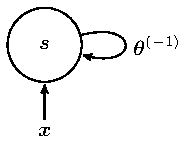
\includegraphics[]{figs/recurrent.pdf}
    \end{center}
    \caption{folded}
    \label{fig:recurrent}
  \end{subfigure}
  \begin{subfigure}[]{.79\textwidth}
    \begin{center}
    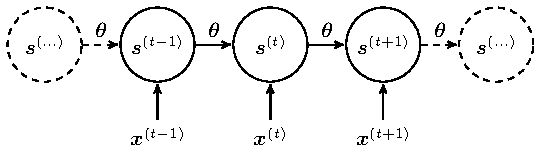
\includegraphics[]{figs/recurrent_uf.pdf}
    \end{center}
    \caption{unfolded}
    \label{fig:recurrent_uf}
  \end{subfigure}
  \caption{Recurrence}
  \label{fig:recurrence}
\end{figure}


\section{Basic RNN}

The functionality of a basic RNN resembles that of a traditional neural network with the addition of a shared hidden state over time.

A RNN can be formulated to predict a sequence as follows:



the abs time of an event is meaningless

\begin{figure}[H]
  \centering
  \begin{subfigure}[]{.2\textwidth}
    \begin{center}
    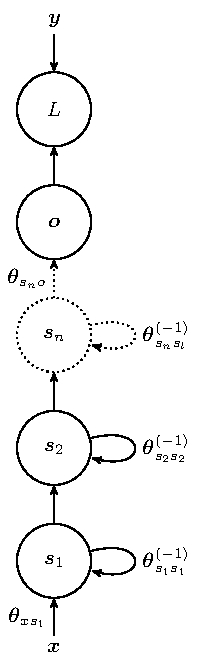
\includegraphics[]{figs/rnn.pdf}
    \end{center}
    \caption{folded}
    \label{fig:rnn_f}
  \end{subfigure}
  \begin{subfigure}[]{.79\textwidth}
    \begin{center}
    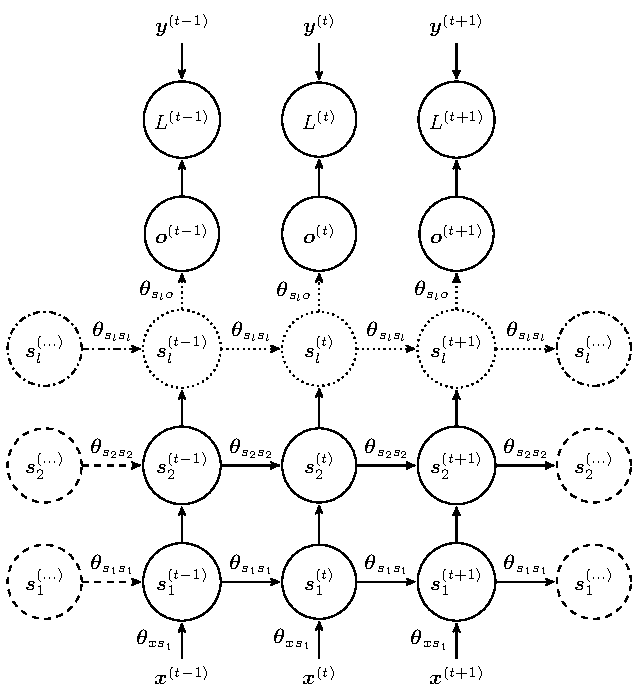
\includegraphics[]{figs/rnn_uf.pdf}
    \end{center}
    \caption{unfolded}
    \label{fig:rnn_uf}
  \end{subfigure}
  \caption{Recurrence}
  \label{fig:rnn}
\end{figure}

%%% Local Variables:
%%% mode: latex
%%% TeX-master: "thesis"
%%% End:
